\documentclass[12pt]{article}
\usepackage{../../template}
\author{niceguy}
\title{Lecture 17}
\begin{document}
\maketitle

\section{Manometers}

\begin{ex}
	Determine an equation for $p_A-p_B$ along the pipe in terms of the specific weight of the folwing fluid $\gamma_1$ in the pipe, the specific weight of the gage fuild $\gamma_2$, and the various heights indicated (Fig~\ref{m1}).

	\begin{figure}
		\centering
		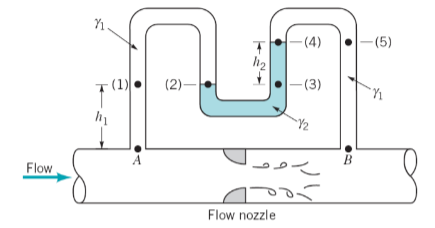
\includegraphics[width=0.7\textwidth]{m1.png}
		\label{m1}
		\caption{Pipe}
	\end{figure}
	$$p_A - h_1\gamma_1 - h_2\gamma_2 + (h_1+h_2)\gamma_1 = p_B$$
	Rearranging,
	$$p_1-p_B = h_2(\gamma_2-\gamma_1)$$
\end{ex}

\begin{ex}
	Inclined tube manometer (Fig~\ref{m2}):

	\begin{figure}
		\centering
		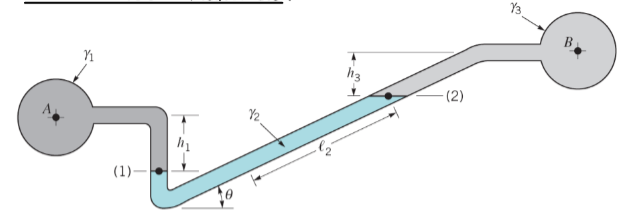
\includegraphics[width=0.7\textwidth]{m2.png}
		\label{m2}
		\caption{Inclined tube manometer}
	\end{figure}

	$$p_A + h_1\gamma_1 - l_2\gamma_2\sin\theta - h_3\gamma_3 = p_B$$
	Rearranging,
	$$p_A - p_B = l_2\gamma_2\sin\theta + h_3\gamma_3 - h_1\gamma_1$$
	If $A$ and $B$ are gases,
	$$p_A - p_B = l_2\gamma_2\sin\theta$$
\end{ex}

\section{Hydrostatic Forces on Submerged Surfaces}

We assume

\begin{itemize}
	\item $\vec{F}_p \perp$ surface
	\item No shear stress
	\item For incompressible fluids at rest, pressure varies linearly with depth
\end{itemize}

\section{Hydrostatic Forces acting on Planar Surfaces}

This can be done by integration.

\begin{ex}
	Find the mass of the gate such that it will open when the water level exceeds 2m (Fig~\ref{gate}). ($\cos\theta=0.6$, width is 1.8m)

	\begin{figure}
		\centering
		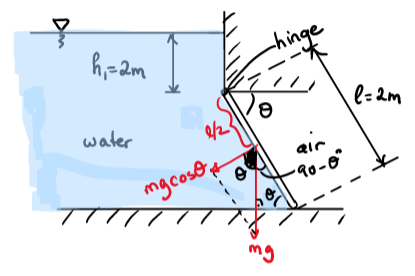
\includegraphics[width=0.7\textwidth]{gate.png}
		\label{gate}
		\caption{Gate}
	\end{figure}

Closing moment:
$$M = \frac{L}{2} \times mg\cos\theta = 0.6mg$$

Opening moment: \\
Defining $x$ as the distance along the gate,
\begin{align*}
	M &= \iint_A xpdA \\
	  &= \int_0^l x\rho ghw dx \\
	  &= \int_0^l x\rho g(h_1+x\sin\theta)w dx \\
	  &= \rho gw \times \frac{18.4}{3} \\
\end{align*}

Equating both yields $m=18400$kg.
\end{ex}


The second method is by using a pressure prism. The average pressure is given by

$$p_{av} = \frac{\rho gh}{2}$$

And the force is then

$$F = \frac{1}{2}\rho gh^2b$$

In the case if pressure is not 0 at the lowest point, the formulae for pressure and force are trivial, and are left to the reader as an exercise. Note that atmospheric pressure can (usually) be ignored as it is cancelled out.

\section{Hydrostatic Force acting on Curved Surfaces}

This can be done through integration.
\begin{ex}
	Find the horizontal force required to hold the gate (Fig~\ref{gate2}) closed. Neglect the mass of the gate. (width = 6m, radius $R$ = 2m)

	\begin{figure}
		\centering
		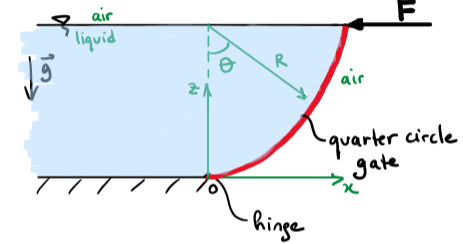
\includegraphics[width=0.7\textwidth]{gate2.png}
		\caption{Gate}
		\label{gate2}
	\end{figure}

	We first paramatrise the curve
	\begin{align*}
		x &= R\sin\theta \\
		z &= R - R\cos\theta
	\end{align*}

	Moment is then
	\begin{align*}
		M &= \int x |dF_z| + z |dF_x| \\
		  &= \int_{\theta = 0}^{\theta = \pi/2} R \sin{\theta} p w \cos{\theta} R d\theta + (R - R\cos{\theta})pw\sin{\theta}R d\theta \\
		  &= \int_0^{\pi/2} Rpw\sin{\theta} R d\theta \\
		  &= \int_0^{\pi/2} R^3 \rho g w \sin{\theta} \cos{\theta} d\theta \\
		  &= R^3 \rho g w \int_0^{\pi/2} \sin{\theta} \cos{\theta} d\theta \\
		  &= R^3 \rho g w \int_0^{\pi/2} \frac{\sin^2{\theta}}{2} d\theta \\
		  &= \frac{R^3 \rho g w}{4} (-\cos{2\theta}) \Big |_{\theta=0}^{\theta=\pi/2} \\
		  &= \frac{R^3 \rho g w}{4} (\cos{0} - \cos{\pi}) \\
		  &= \frac{R^3 \rho g w}{2}
	\end{align*}
	Then the force is
	$$\frac{R^2\rho gw}{2} = 120000\text{N}$$
\end{ex}

The second method is to parametrise the surface.

\begin{ex}
\begin{align*}
	x &= R\sin\theta \\
	z &= R - R\cos\theta \\
	y &= y
\end{align*}

Then
$$\vec{r} = R\sin\theta\hat{i} + y\hat{j} + (R-R\cos\theta)\hat{i}$$
giving
$$\vec{r}_\theta = R\cos\theta\hat{i} + R\sin\theta\hat{k}$$
and
$$\vec{r}_y = \hat{j}$$
so
$$\vec{r}_\theta\times\vec{r}_y = -R\sin\theta\hat{i} + R\cos\theta\hat{k}$$
whose magnitude is $R$. The moment is then

\begin{align*}
	M_y &= \int_S x|dF_z| + z|dF_x| \\
	    &= \iint R\sin\theta(pR\cos\theta)dyd\theta + \iint(R-R\cos\theta)pR\sin\theta dyd\theta
\end{align*}
which gives the same integral as above.
\end{ex}
\end{document}
